% MA211 - Lecture 03
\documentclass[pdftex, xcolor=pdftex, dvipsnames,handout]{beamer}

\usetheme{MA211}
\usepackage{thumbpdf}
\usepackage{wasysym}
%\usepackage{ucs}
\usepackage[utf8]{inputenc}
\usepackage{pgf,pgfarrows,pgfnodes,pgfautomata,pgfheaps,pgfshade}
\usepackage{verbatim}

\usepackage{eurosym}
\usepackage{euler}

\usepackage{calc}               % Simple computations with LaTeX variables
%\usepackage[hang]{caption2}     % Improved captions

\usepackage{graphicx}           % Standard graphics package

\usepackage{amsmath, amsthm, amssymb}


\newcommand{\fquad}{\mbox{\qquad}}
\newcommand{\bull}{$\bullet$ }

\newcommand {\I} {\mathcal I}
\newcommand {\calI} {\mathcal I}
\def\disint{\displaystyle\int}

\DeclareMathOperator{\D}{d}
\newcommand{\dydx}{\frac{\D y}{\D x}}

%\definecolor{gray}{rgb}{0.69, 0.69, 0.69} \newcommand{\gray}[1]{\textcolor{gray}{#1}}
\definecolor{dogreen}{rgb}{0.33, 0.42, 0.18} \newcommand{\dogreen}[1]{\textcolor{dogreen}{#1}}
\definecolor{maroon}{rgb}{.5,0.2,0.2}\newcommand{\maroon}[1]{\textcolor{maroon}{#1}}
\definecolor{greena}{rgb}{.1,0.581,0.1}\newcommand{\greena}[1]{\textcolor{greena}{#1}}

\definecolor{blue4}{rgb}{0,0,.545}
\newcommand{\Blue}[1]{\textcolor{blue}{#1}}
\newcommand{\Red}[1]{\textcolor{red}{#1}}
\definecolor{pink}{rgb}{1.,0.75,0.8}
\definecolor{darkred}{rgb}{0.5,0.0,0.0}
\definecolor{darkgreen}{rgb}{0,0.3,0.3}
\definecolor{purple}{rgb}{0,0.3,0.3}
\definecolor{darkblue}{rgb}{0.0, 0.0, .5}
\definecolor{dpurple}{rgb}{.3,.0,.3}
\newcommand{\Green}[1]{\textcolor{darkgreen}{#1}}
\newcommand{\DRed}[1]{\textcolor{darkred}{#1}}
\newcommand{\DBlue}[1]{\textcolor{darkblue}{#1}}
\newcommand{\Purple}[1]{\textcolor{dpurple}{#1}}
\newcommand{\Emph}[1]{\textcolor{darkred}{\textbf{\it #1}}}
\newcommand{\remph}[1]{\textcolor{darkred}{\textbf{\emph{#1}}}}
\newcommand{\bemph}[1]{\textcolor{darkblue}{\textbf{\emph{#1}}}}
\newcommand{\gemph}[1]{\textcolor{darkgreen}{\textbf{\emph{#1}}}}
\newcommand{\Bf}[1]{\textcolor{darkblue}{\textbf{#1}}}
\newcommand{\Gf}[1]{\textcolor{darkgreen}{\textbf{#1}}}
\newcommand{\Rf}[1]{\textcolor{red}{\textbf{#1}}}
\newcommand{\Rmf}[1]{\textcolor{red}{\mathbf{#1}}}

\newcommand{\Conj}[1]{\overline{#1}}

\newcommand{\code}[1]{\textcolor{darkblue}{\texttt{\textbf{#1}}}}
\newcommand{\icode}[1]{{\blue\texttt{\textbf{\emph{#1}}}}}
\newcommand{\gcode}[1]{{\Green{\texttt{\textbf{\emph{#1}}}}}}
\newcommand{\out}[1]{\texttt{\emph{\textbf{\Green{#1}}}}}





\newenvironment{vminipage}%
{\begin{Sbox}\begin{minipage}\begin{small}\begin{verbatim}}%
{\end{verbatim}\end{small}\end{minipage}\end{Sbox}\fbox{\TheSbox}}

\newenvironment{nminipage}%
{\begin{Sbox}\begin{minipage}}%
{\end{minipage}\end{Sbox}\fbox{\TheSbox}}


\let\Arg\relax\DeclareMathOperator{\Arg}{\mathtt{Arg}}
\let\Arg\relax\DeclareMathOperator{\e}{\mathtt{e}}

\newcommand {\AND} {\wedge}
\newcommand {\OR} {\vee}
\newcommand {\NOT} {\neg}
\newcommand {\IMPLIES} {\rightarrow}
%\newcommand {\IFF} {\leftrightarrow}
\renewcommand {\iff} {\Leftrightarrow}
\newcommand {\NAND} {\uparrow}
\newcommand {\NOR} {\downarrow}
\newcommand {\XOR} {\otimes}

\newenvironment{citemize}% Colour items
{\begin{description}}%
{\end{description}}

\newcommand {\maroonitem}{\item[\maroon{$\bullet$}]}

\newcommand {\gitem} {\item {\includegraphics[width=.4cm,angle=-10]{img/green-bullet-on-white.ps}}}
\newcommand {\ritem} {\item {\includegraphics[width=.4cm,angle=-10]{img/red-bullet-on-white.ps}}}
\newcommand {\yitem} {\item {\includegraphics[width=.4cm,angle=-10]{img/yellow-bullet-on-white.ps}}}
\newcommand {\bitem} {\item {\includegraphics[width=.4cm,angle=-10]{img/blue-bullet-on-white.ps}}}

\newcommand {\greenitem} {\item {\includegraphics[width=.4cm,angle=-10]{img/green-bullet-on-white.ps}}}
\newcommand {\reditem} {\item {\includegraphics[width=.4cm,angle=-10]{img/red-bullet-on-white.ps}}}
\newcommand {\yellowitem} {\item {\includegraphics[width=.4cm,angle=-10]{img/yellow-bullet-on-white.ps}}}
\newcommand {\blueitem} {\item {\includegraphics[width=.4cm,angle=-10]{img/blue-bullet-on-white.ps}}}

\newcommand {\eq}[1]%
  {$\DBlue{#1}$}
\newcommand {\eqd}[1]%
  {$\displaystyle\DBlue{#1}$}
%\newcommand{\eq}[1]{\boldmath \DBlue{$#1$}}


\newcommand {\csf}{\centerslidesfalse}
\newcommand {\cst}{\centerslidestrue}

\newcommand {\vecii}[2] {   \big(\begin{smallmatrix} #1 \\ #2 \end{smallmatrix}\big)}
\newcommand{\atwo}[2]{\left(\!\!\begin{array}{c} #1 \\ #2 \end{array}\!\!\right)}


\newcommand{\C}{\mathbb{C}}
\newcommand{\Q}{\mathbb{Q}}
\newcommand{\R}{\mathbb{R}}
\newcommand{\N}{\mathbb{N}}
\newcommand{\Z}{\protect\mathbb{Z}}  % protect for index.
\newcommand {\Rs}{ \mathbb{R}}
\newcommand {\Cs}{ \mathbb{C}}
\newcommand {\Rnn}{ \mathbb{R}^{n \times n}}
\newcommand {\Rn}{ \mathbb{R}^{n}}


\newcommand{\mblock}{%
\setbeamercolor*{block title}{bg=maroon,fg=white}
\setbeamercolor*{block body}{bg=white,fg=maroon}
}%

\newcommand{\bblock}{%
\setbeamercolor*{block title}{bg=Steel,fg=white}
\setbeamercolor*{block body}{bg=Mylightgray,fg=Steel}
}%

\newcommand{\gblock}{%
\setbeamercolor*{block title}{bg=Green,fg=white}
\setbeamercolor*{block body}{bg=Mylightgray,fg=darkgreen}
}%


\newcommand{\rblock}{%
\setbeamercolor*{block title}{bg=Red,fg=white}
\setbeamercolor*{block body}{bg=white,fg=Black}
}%


\newcommand{\TakeNotes}{
\includegraphics[width=2cm]{TakeNote}}


\def\eps{\varepsilon}
\newcommand {\del}[2]{ {\frac{\partial #1}{\partial #2}}}
\newcommand {\x}[1]{x^{[#1]}}
\newcommand {\delx}{ {\frac{\partial}{\partial x}}}
\newcommand {\delt}{ {\frac{\partial}{\partial t}}}
\newcommand {\dely}{ {\frac{\partial}{\partial y}}}
\newcommand {\ith}{{(i)}}
\renewcommand {\vec}[1]{ {\boldsymbol{#1}}}
\newcommand {\Oh} {\mathcal O}
\newcommand {\Err} {\mathcal E}
%\newcommand {\th} {\mathrm{th}}
\DeclareMathOperator{\fl}{fl}
\DeclareMathOperator{\sign}{sign}
\DeclareMathOperator{\Cond}{Cond} 
\DeclareMathOperator{\cond}{cond}
\DeclareMathOperator{\diag}{diag} 
\DeclareMathOperator{\sym}{sym} 
\DeclareMathOperator{\Trace}{Trace}
\DeclareMathOperator{\E}{e}

\newcommand {\Rsym}{{ \mathbb{R}^{n \times n}_\mathrm{sym}}}

\parskip .25cm


\theoremstyle{definition}
\newtheorem{exercise}{Exercise}[section]
\newtheorem{method}{Method}[section]



\subtitle{MA211}
\title{Lecture 3: Limits}

\author{Dr Niall Madden}

\date{\Large Monday 15 September 2008}


\begin{document}


\frame{

\begin{block}{}
\begin{center}
{\large \insertsubtitle}

\vspace{.1cm}

\begin{Large}
\textbf{\inserttitle}
\end{Large}

\vspace{.15cm}

{\footnotesize \insertauthor}

\vspace{.4cm}

{ {\insertdate}}
\end{center}
\end{block}


\vspace{-0.25cm}
\begin{center}
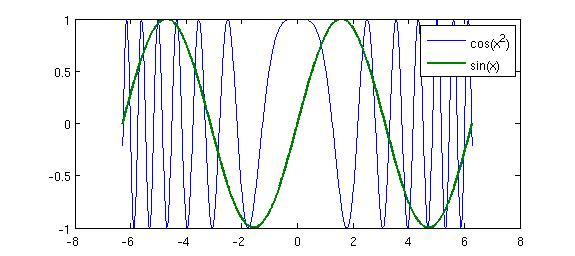
\includegraphics[height=4cm]{CosSin}
\end{center}
}



%\section{Outline}
\frame{
  \frametitle{Outline}
 \tableofcontents



}


\frame{

\begin{center}
{\Large \Bf{Problem Solving Sessions}}
\end{center}

Problem Solving sessions (tutorials) will start next week. There will
be three per week. Attend whichever one you like
\begin{itemize}

\item Tuesday, 3pm, AC202

\item Wednesday, 5pm, QA003 (Physiology lecture room)

\item \alert{????? (Thursday, 6pm, IT207??)}
\end{itemize}

}



\section{Recall... }
\subsection{Domain, Codomain and Range}
\frame{

\begin{block}{}
A a \Bf{function} \eq{f} from a set \eq{X} to a set \eq{Y} is a rule of
correspondences that associates every element of \eq{X} with some
(single)  element of \eq{Y}. We write:
\[
f: X \rightarrow Y.
\]
\end{block}




\begin{itemize}
\item \eq{X} is called the \Bf{Domain} of \eq{f}, and 

\item \eq{Y} is called the \Emph{Codomain}.

\item the \Emph{Range} of \eq{f} the subset of \eq{Y} that contains
  all the elements of \eq{Y}   that are the image under \eq{f} of some
element of \eq{X}. 
\end{itemize}


}

\section{One-to-one and Onto}
\subsection{One-to-one}
\frame{

A function from \eq{X} to \eq{Y}  is \Emph{One-to-One} if no two
elements of \eq{X} are mapped to the same element of \eq{Y}. (In some
books this is called \Emph{injective}).

\begin{definition}[One-to-one]
The function \eq{f:X \rightarrow Y} is one-to-one  if
whenever \eq{f(x_1)= f(x_2)}  then \eq{x_1 =x_2}.
\end{definition}

\vspace{3cm}
}


\frame{

\begin{example}
Is the function  \eq{f:\R \rightarrow \R} given by \eq{f(x)=x^2} is
one-to-one? Why?

~

Find other sets \eq{X \subseteq \R} and \eq{Y \subseteq \R} such that 
 \eq{f: X \rightarrow Y} is one-to-one.
\end{example}


\vspace{3cm}


}

\subsection{Onto}


\frame{
A function from \eq{X} to \eq{Y}  is \Emph{onto} if every element of
\eq{Y} is the image of some element of \eq{X}. (In some
books this is called \Emph{surjective}).

\begin{definition}[Onto]
The function \eq{f:X \rightarrow Y} is onto if for each $y \in B$
there exists $x \in A$ such that $y$ is the image of $x$. That is
\[
\forall y \in B, \exists x \in A \text{ such that } f(x) =y.
\]
\end{definition}

A third way of expressing this is by saying the \Emph{range} of \eq{f}
is equal to its \emph{codomain}.


}

\frame{

\begin{example}
Show that the function  \eq{f:\R \rightarrow \R} given by \eq{f(x)=x^2} is
not \Bf{onto}.

~

Find other sets \eq{X \subseteq \R} and \eq{Y \subseteq \R} such that 
 \eq{f: X \rightarrow Y} is onto.
\end{example}


\vspace{3cm}


}

\frame{

\begin{exercise}[3.1]
Give an example of a function:
\begin{enumerate}[(i)]
\item  $f:\Z \rightarrow \N$ that is onto but \emph{not} one-to-one.

~

\item  $f:\N \rightarrow \N$ that is one-to-one, but not onto.

\end{enumerate}

\end{exercise}
}

\section{Inverse functions}



\frame{
When a function is both \alert{one-to-one} and \alert{onto} is has an
\Bf{Inverse}.

\begin{definition}[Inverse]
If the function \eq{g} is the \alert{inverse} of \eq{f} then 
\[
\text{ when } f(x)=y, \text{ we get that } g(y)=x.
\]

Usually we write \eqd{g=f^{-1}}.
\end{definition}

\Emph{Examples:}

\vspace{2cm}

}

\subsection{Properties of Inverse Functions}

\frame{

\begin{enumerate}

\item \eq{ y = f(x) ~~  \Longleftrightarrow  ~~x = f^{-1}(y)}

~

\pause\item The domain of \eq{f^{-1}} is the range of \eq{f}
\item The range of \eq{f^{-1}} is the domain of \eq{f}

~

\pause\item  \eq{f^{-1}\big(f(x)\big) =x}
\item \eq{f\big(f^{-1}(x)\big) =x}

~

\pause \item \eq{\big(f^{-1}\big)^{-1}=f}.

~

\pause \item The graph of \eq{f^{-1}} is the reflection of the graph of
\eq{f} in the line \eq{x=y}.


\end{enumerate}

}



\section{The trigonometric functions}
\frame{

You'll remember the definition of \eq{\cos} and \eq{\sin} in terms of
a right-angle triangle.

Here is another, equivalent definition.

\begin{itemize}

\item Take the usual coordinate axes centred on $(0,0)$ and draw the
  unit circle,
\item Mark   the point $(1,0)$.

\item Trace an arc of length \eq{t} \Emph{anti-clockwise} from $(1,0)$
  along the circle. Call the point at the end of that arc \eq{P}.

\item The \eq{x}-coordinate of \eq{P} is \eq{\cos(t)} and the
  \eq{y}-coordinate is \eq{\sin(t)}.

\end{itemize}

}


\frame{

\begin{center}
{\Large \Bf{The $\cos$ (top) and $\sin$ (bottom) functions}}

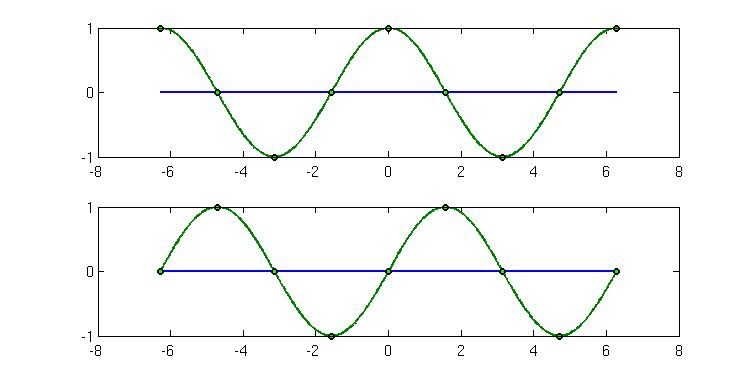
\includegraphics[width=12cm]{cos}
\end{center}

}

\frame{

\begin{exercise}[3.2]
Find subsets \eq{X} and \eq{Y} of the real numbers such that the
functions \eq{f:X \rightarrow Y} are \Emph{invertible}
(i.e., both \emph{one-to-one} and \emph{onto}) for
\begin{enumerate}[(i)]
\item \eq{f(x) = \sin(x)}
\item \eq{f(x) = \cos(x^2)}
 \end{enumerate}
\end{exercise}
}


\section{Limits}
\frame{

\begin{block}{}
When we write 
\[
\lim_{x \rightarrow c} f(x) = L
\]
or say ``\emph{The limit of \eq{f} as \eq{x} approaches \eq{c} is
  \eq{L}}'' we mean that we can make \eq{f} as close to \eq{L} as we
  would like by taking \eq{x} as close to \eq{c} as is needed.
\end{block}

\pause

\begin{definition}[Limit]
If for any \eq{\eps>0}, no matter how small, we can find \eq{\delta>0}
such that
\[
|f(x) -L | < \eps ~~ \text{ when  } ~~ |x-c| < \delta.
\]
then we can say
\[
\lim_{x \rightarrow c} f(x) = L.
\]
\end{definition}
}

\frame{

\begin{example}
Show that 
\[
\lim_{x\rightarrow 3} (2x+1)=7.
\]
\end{example}

\vspace{4cm}

}

\frame{


\begin{exercise}[3.3]
Show \emph{carefully} that 
\begin{enumerate}[(i)]
\item \eq{\lim_{x \rightarrow 4} 3x-7=5.}
\item \eqd{\lim_{x \rightarrow 2} \big(\frac{x}{2}+3\big)} is \eq{4}
\end{enumerate}
\end{exercise}
}

\frame{
Calculating the limit of a given function as it approaches a certain
point is a fairly standard task.

\begin{example}
Find the limit of 
\[
f(x) = \frac{2x^2 -3x-2}{x-2}
\]
as \eq{x} approaches 2.
\end{example}

}



\subsection{Important Properties}
\frame{
Let \eq{n} be an integer, \eq{k} a constant real number, and \eq{f}
and \eq{g} be functions that have a limit at \eq{c}. Then
\begin{enumerate}[<+->]
\item $\displaystyle\lim_{x \rightarrow c} k = k$;

~

\item \eq{\displaystyle\lim_{x \rightarrow c} x = c};

~

\item $\displaystyle\lim_{x \rightarrow c} kf(x) = k\lim_{x \rightarrow c} f(x)$;

~

\item $\displaystyle\lim_{x \rightarrow c} \big(f(x) + g(x)\big) = 
\lim_{x \rightarrow c} f(x) + \lim_{x \rightarrow c} g(x)$.

~

\item $\displaystyle\lim_{x \rightarrow c} \big(f(x) - g(x)\big) =
\lim_{x \rightarrow c} f(x) - \lim_{x \rightarrow c} g(x)$.
\end{enumerate}
}

\frame{
\begin{enumerate}[<+->]
\setcounter{enumi}{6}
\item $\displaystyle\lim_{x \rightarrow c} \big(f(x) \cdot g(x)\big) = 
\lim_{x \rightarrow c} f(x) \cdot \lim_{x \rightarrow c} g(x)$.

~

\item $\displaystyle
  \lim_{x \rightarrow c} \frac{f(x)}{g(x)} = 
\frac{\lim_{x \rightarrow c} f(x)}{\lim_{x \rightarrow c} g(x)}.
\pause \quad \text{ \Emph{providing that} } \quad \lim_{x \rightarrow c} g(x)
  \neq 0$.
\pause

~

\item $\displaystyle
  \lim_{x \rightarrow c} \bigg( f(x) \bigg)^n = 
\bigg( \lim_{x \rightarrow c} f(x) \bigg)^n$.

~

\item $\displaystyle
  \lim_{x \rightarrow c} \bigg( f(x) \bigg)^{(1/n)} = 
\bigg( \lim_{x \rightarrow c} f(x) \bigg)^{(1/n)}$.



\end{enumerate}
}


\frame{

There are many neat tricks for computing limits, particularly those of
the form
\[
  \lim_{x \rightarrow c} \frac{f(x)}{g(x)} = 
\frac{\lim_{x \rightarrow c} f(x)}{\lim_{x \rightarrow c} g(x)}.
\pause \quad \text{ where  } \quad \lim_{x \rightarrow c} g(x)
  = 0
\]

One of these is \Emph{The Squeeze Theorem}, but even better is
l'Hopital's Rule

We'll cover these on Wednesday.
}

\end{document}
\subsection{The Squeeze Theorem}

\frame{

\begin{theorem}[The Squeeze Theorem]
Let \eq{f}, \eq{g} and \eq{h} be functions such that 
\[
f(x) \leq g(x) \leq h(x) \quad \text{ for } x \text { near } c.
\]
If
\[ 
\lim_{x \rightarrow c} f(x) = L \quad \text{ and } 
\lim_{x \rightarrow c} h(x) = L,
\]
then 
\[ \lim_{x \rightarrow c} g(x) = L.
\]
\end{theorem}

}

\frame{
\begin{example}
Use the Squeeze Theorem to show that
\[
\lim_{t \rightarrow 0} \frac{\sin(t)}{t} = 1.
\]
\end{example}

\vspace{4cm}


}



\frame{

\begin{exercise}[3.4]

Use the Squeeze theorem to answer the following questions.
\begin{enumerate}[(i)]
\item Find  \eq{\lim_{x \rightarrow 0} f(x)} if  $f$ is a function such that 
\[ 2-x^2 \leq f(x) \leq 2\cos(x),\]


\item If $\lim_{t \rightarrow 0} |f(t)|=0$, show that  $\lim_{x \rightarrow
    0} f(t)=0$.

\item What is the largest possible domain of  $f(t)=t\sin(1/t)$?

Evaluate  \eq{\lim_{t\rightarrow 0} f(t)}.


\end{enumerate}

\end{exercise}
}

\subsection{l'Hopital's Rule}
\frame{
The rule of l'Hopital is




\begin{block}{}
\[
\frac{\lim_{x \rightarrow c}  f(x)}{\lim_{x \rightarrow c}  g(x)} = 
\frac{\lim_{x \rightarrow c} f'(x)}{\lim_{x \rightarrow c} g'(x)}
\]
\end{block}
where here, for example,  \eq{f'(x)} is the \alert{derivative} of \eq{f} with
respect to \eq{x}.

And explaining what that means is one of the real reasons we've
introduced the idea of a limit.


}

\section{Derivatives}
\frame{
How can you calculate the slope of the tangent to a function \eq{f} at a
given point \eq{x}?

One approach is to compute the slope of the line that intersects 
the function at \eq{x} and some near by point \eq{x+h}. (This is
called a  \Emph{secant} line)...

And then get the limit of the slope of the secant lines as \eq{h}
tends to zero.

This gives us the definition
\begin{block}{}
\[
f'(x) :=  \frac{d}{dx}f(x) := \lim_{h \rightarrow 0} \frac{ f(x+h) -
  f(x)}{h}.
\]
\end{block}

}

\frame{
\begin{example}
Find the derivative of $f(x)=x^2$ using the above definition. (i.e,
``\emph{differentiate \eq{f(x)=x^2} from first principles}.'').
\end{example}

\vspace{4cm}
}

\frame{
\begin{example}
Find the derivative of $f(x)=1/x$ from first principles.
\end{example}
\vspace{4cm}

}




\frame{

\begin{exercise}[3.5]
From first principles, find the derivative of 
\begin{enumerate}
\item \eqd{f(x)= \frac{1}{3} x^3.}
\item \eqd{f(x)= x^n} for any $n=1, 2, 3, ...$
\item \eqd{f(x)  x^{-n}}

\end{enumerate}
\end{exercise}

For a hint for Part (ii), use the \Emph{binomial theorem}....
}


\frame{
\emph{Hint for Exer 3.5:}  Recall \Emph{Binomial Expansion}
\[ 
 (a  +  b)^n  =  a^n + \binom{n}{1}a^{n-1}b
+ \binom{n}{2}a^{n-2}b^2 + \cdots + \binom{n}{n-1}ab^{n-1} + b^n
\]
\pause
\[ 
 (a  +  b)^n  =
\sum_{k=0}^n
  \binom{n}{k}  a^{n-k}  b^k,
\]
Here  the  \Emph{Binomial  Coefficient}
  $\binom{n}{k}$   (``$n$  choose   $k$'')  is   
\[
  \binom{n}{k}  =  \frac{n!}{k!\,  (n-k)!},  
\]
and   $n!$  (``$n$  factorial'') is $n! = n \cdot (n-1) \dots 3 \cdot 2
\cdot 1$.


}



\end{document}
